\documentclass[
11pt, % Set the default font size, options include: 8pt, 9pt, 10pt, 11pt, 12pt, 14pt, 17pt, 20pt
%t, % Uncomment to vertically align all slide content to the top of the slide, rather than the default centered
%aspectratio=169, % Uncomment to set the aspect ratio to a 16:9 ratio which matches the aspect ratio of 1080p and 4K screens and projectors
]{beamer}

\graphicspath{{Images/}{./}} % Specifies where to look for included images (trailing slash required)

\usepackage{todonotes}
\usepackage{graphicx}
\usepackage{xcolor}
\usepackage{subfig}
%%\usepackage[noend]{algpseudocode}

%
%\usepackage{algorithm}
%\usepackage{algorithmic}
\usepackage{algorithm}
\usepackage{algpseudocode}
\usepackage{blkarray}
\usepackage{amsmath}
\usepackage{xspace}
\usepackage{float}


\usepackage{tikz}
\usetikzlibrary{matrix, decorations, patterns, positioning, shapes, calc, intersections, arrows, fit}

\usetikzlibrary{patterns}
\usetikzlibrary{fit,calc,positioning,decorations.pathreplacing,matrix,3d, hobby}

\usepackage{booktabs} % Allows the use of \toprule, \midrule and \bottomrule for better rules in tables
\usepackage{bm}
\usepackage{multirow}
\usepackage{ragged2e}


\newcommand{\brown}[1]{{\color{brown} #1 }}

%% Colors from https://latexcolor.com/
\definecolor{pastelviolet}{rgb}{0.8, 0.6, 0.79}
\definecolor{babyblueeyes}{rgb}{0.63, 0.79, 0.95}
\definecolor{pastelyellow}{rgb}{0.99, 0.99, 0.59}
\definecolor{pastelgreen}{rgb}{0.47, 0.87, 0.47}
\definecolor{pastelred}{rgb}{1.0, 0.41, 0.38}
\colorlet{patternblue}{blue!60}



%%\newcommand{\tensorcolor}{patternblue}
\newcommand{\tensorcolor}{cyan}


\colorlet{darkred}{red!80!black}
\colorlet{darkblue}{blue!80!black}
\newcommand<>{\darkred}[1]{{\color{darkred}{#1}}}
\newcommand<>{\darkblue}[1]{{\color#2{blue!50!black!100}{#1}}}

\newcommand{\A}{\mathbf{A}}
\newcommand{\B}{\mathbf{B}}
\newcommand{\CC}{\mathbf{C}}
%\newcommand{\Real}{\mathbb{R}}
\newcommand{\vc}[1]{\bm{#1}}

\usetheme{Madrid}

%\newcommand{\Tra}{{\sf T}} 


%\newcommand{\Ms}[2]{\mathbf{#1}^{(#2)}} 
%\newcommand{\M}[1]{\mathbf{#1}} 
%\newcommand{\Mb}[2]{\mathbf{#1}_{#2}} 
%\newcommand{\Mbs}[3]{\mathbf{#1}_{#2}^{(#3)}} 

%\usepackage{enumitem}

%% ------------------------------------------------------------
%% PACKAGES
%% ------------------------------------------------------------

%% For \circledast
\usepackage{amssymb,amsfonts,amsmath}

%% For \mathscr
\usepackage[mathscr]{eucal}

%% For \llbracket and \rrbracket, \varoast, \varoslash
\usepackage{stmaryrd}

%% For \boldsymbol
\usepackage{amsbsy}

%% For \bm (bold math)
\usepackage{bm}

%% For \set, \Set
\usepackage{braket}

%% ------------------------------------------------------------
%% MACROS
%% ------------------------------------------------------------


%% --- Extras ---
% Transpose
\newcommand{\Tra}{{\sf T}} 
\newcommand{\parens}[1]{(#1)}
\newcommand{\Parens}[1]{\left(#1\right)}
\newcommand{\dsquare}[1]{\llbracket #1 \rrbracket}
\newcommand{\Dsquare}[1]{\left\llbracket #1 \right\rrbracket}
\newcommand{\curly}[1]{\{ #1 \}}
\newcommand{\Curly}[1]{\left\{ #1 \right\}}
\newcommand{\Real}{\mathbb{R}}
\newcommand{\qtext}[1]{\quad\text{#1}\quad}

%% --- Vectors ---
% vector
\newcommand{\V}[2][]{{\bm{#1\mathbf{\MakeLowercase{#2}}}}} 
% element of vector
\newcommand{\VE}[3][]{#1{\MakeLowercase{#2}}_{#3}} 
% vector in series
\newcommand{\Vn}[3][]{{\bm{#1\mathbf{\MakeLowercase{#2}}}}^{(#3)}} 
% transposed vector in series
\newcommand{\VnTra}[3][]{{\bm{#1\mathbf{\MakeLowercase{#2}}}}^{(#3)\Tra}} 
% element of vector in series
\newcommand{\VnE}[4][]{#1{\MakeLowercase{#2}}^{(#3)}_{#4}} 

%% --- Matrices ---
% matrix
\newcommand{\M}[2][]{{\bm{#1\mathbf{\MakeUppercase{#2}}}}} 
% matrix in series
\newcommand{\Mn}[3][]{{\bm{#1\mathbf{\MakeUppercase{#2}}}}^{(#3)}} 
% transposed matrix in series 
\newcommand{\MnTra}[4][]{{\bm{#1\mathbf{\MakeUppercase{#2}}}}^{(#3)\Tra}} 
% matrix column
\newcommand{\MC}[3][]{\V[#1]{#2}_{#3}} 
% column of matrix in series
\newcommand{\MnC}[4][]{\Vn[#1]{#2}{#3}_{#4}} 
% transposed column of matrix in series
\newcommand{\MnCTra}[4][]{\VnTra[#1]{#2}{#3}_{#4}} 
% matrix element
\newcommand{\ME}[3][]{#1{\MakeLowercase{#2}}_{#3}} 
% element of matrix in series
\newcommand{\MnE}[4][]{#1{\MakeLowercase{#2}}^{(#3)}_{#4}} 

%% --- Tensors ---
% tensor
\newcommand{\T}[2][]{\boldsymbol{#1\mathscr{\MakeUppercase{#2}}}} 
% tensor slide
\newcommand{\TS}[3][]{\M[#1]{#2}_{#3}}
% tensor element
\newcommand{\TE}[3][]{#1{\MakeLowercase{#2}}_{#3}}
% matriczied tensor
\newcommand{\Mz}[3][]{\M[#1]{#2}_{(#3)}}

%% --- Operators ---
% outer product
\newcommand{\Oprod}{\circ} 
% Kronecker product
\newcommand{\Kron}{\otimes} 
% Khatri-Rao product
\newcommand{\Khat}{\odot} 
% Hadamard (elementwise multiply)
\newcommand{\Hada}{\ast} 
\newcommand{\BigHada}{\mathop{\mbox{\fontsize{18}{19}\selectfont $\circledast$}}} 
% Elementwise divide
\newcommand{\Divi}{\varoslash}





%----------------------------------------------------------------------------------------
%	PRESENTATION INFORMATION
%----------------------------------------------------------------------------------------

\title[Low rank approximations]{Low rank approximations for tensors} % The short title in the optional parameter appears at the bottom of every slide, the full title in the main parameter is only on the title page

%\subtitle{Optional Subtitle} % Presentation subtitle, remove this command if a subtitle isn't required

\author[Suraj Kumar]{Suraj Kumar} % Presenter name(s), the optional parameter can contain a shortened version to appear on the bottom of every slide, while the main parameter will appear on the title slide

\institute[Inria \& ENS Lyon]{Inria \& ENS Lyon \\ \smallskip Email:\textit{suraj.kumar@inria.fr}} % Your institution, the optional parameter can be used for the institution shorthand and will appear on the bottom of every slide after author names, while the required parameter is used on the title slide and can include your email address or additional information on separate lines

\date[CR12]{CR12: October 2023\\ \smallskip\small https://surakuma.github.io/courses/daamtc.html} % Presentation date or conference/meeting name, the optional parameter can contain a shortened version to appear on the bottom of every slide, while the required parameter value is output to the title slide

%----------------------------------------------------------------------------------------

\begin{document}
	
	%----------------------------------------------------------------------------------------
	%	TITLE SLIDE
	%----------------------------------------------------------------------------------------
	
	\begin{frame}
		\titlepage % Output the title slide, automatically created using the text entered in the PRESENTATION INFORMATION block above
	\end{frame}

\begin{frame}{Properties of matrix Frobenius norm for real matrices}
	\small 
	$$||A||_F^2 = \sum_{i,j}A^2(i,j) = Trace(AA^T) = Trace(A^TA)$$
	\vfill
	$$||A+B||_F^2 = ||A||_F^2 + ||B||_F^2 + 2 \langle A, B \rangle_F$$
	
	Here $\langle A, B \rangle_F$ is known as Frobenius inner product and defined as $\langle A, B \rangle_F = Trace(A^TB) = Trace(B^TA)$.
	
	\vfill
	If $Q$ is an orthonormal matrix then,
	
	$$||A||_F^2  = ||QQ^TA||_F^2 + ||(I-QQ^T)A||_F^2\text,$$
	$$||Q^TA||_F = ||QQ^TA||_F \le ||A||_F \text,$$
	$$\langle A-QQ^TA, QQ^T \rangle_F = 0\text,$$
	$$||QC||_F = ||C||_F \text.$$
	
\end{frame}

\begin{frame}{Singular Value Decomposition (SVD)}
	\small
	\begin{itemize}
		\item It decomposes a matrix $A$ $\in$ $\mathbb{R}^{m \times n}$ to the form $U\Sigma V^T$
		\begin{itemize}
			\item $U$ is an $m\times m$ orthogonal matrix
			\item $V$ is an $n\times n$ orthogonal matrix
			\item $\Sigma$ is an $m\times n$ rectangular diagonal matrix
		\end{itemize}
		\vfill
		\item The diagonal entries $\sigma_i=\Sigma_{ii}$ of $\Sigma$ are called singular values
		\begin{itemize}
			\item $\sigma_i\ge 0$ and $\sigma_1\le \sigma_2\le \cdots \le \sigma_{\min(m,n)}$
		\end{itemize}
		\vfill
		\item The largest $r$ such that $\sigma_r\ne 0$ is called the rank of the matrix
		\vfill
		\item SVD represents a matrix as the sum of $r$ rank one matrices
	\end{itemize}
	\vfill
	\begin{center}
		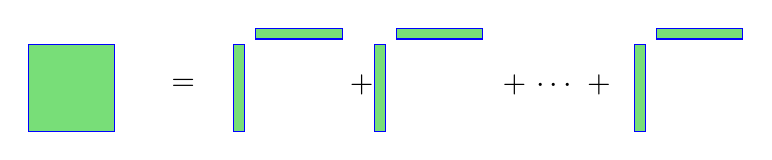
\begin{tikzpicture}[scale=0.275, every node/.style={transform shape}]
		\pgfmathsetmacro{\cubex}{4}
		\pgfmathsetmacro{\cubey}{4}
		\pgfmathsetmacro{\cubez}{4}
		\draw[blue,fill=pastelgreen] (0,0,0) -- ++(-\cubex,0,0) -- ++(0,-\cubey,0) -- ++(\cubex,0,0) -- cycle;
		%%\draw[blue,fill=pastelgreen] (0,0,0) -- ++(0,0,-\cubez) -- ++(0,-\cubey,0) -- ++(0,0,\cubez) -- cycle;
		%%\draw[blue,fill=pastelgreen] (0,0,0) -- ++(-\cubex,0,0) -- ++(0,0,-\cubez) -- ++(\cubex,0,0) -- cycle;
		
		\node[draw=none, text=black, scale=4] at (2,-3,-3) {$=$};
		\pgfmathsetmacro{\smallwidth}{0.5}
		\draw[blue,fill=pastelgreen] (\cubex+2,0,0) -- ++(-\smallwidth,0,0) -- ++(0,-\cubey,0) -- ++(\smallwidth,0,0) -- cycle;
		\draw[blue,fill=pastelgreen] (\cubex+2 +\cubex + 0.5,0.75,0) -- ++(-\cubex,0,0) -- ++(0,-\smallwidth,0) -- ++(\cubex,0,0) -- cycle;
		%%\draw[blue,fill=pastelgreen] (\cubex+2,0.5,0) -- ++(-\smallwidth,0,0) -- ++(0,0,-\cubez) -- ++(\smallwidth,0,0) -- cycle;
		
		\node[draw=none, text=black, scale=4] at (2+\cubex+4.25,-3,-3) {$+$};
		
		\draw[blue,fill=pastelgreen] (\cubex+2.5 + \cubex+2,0,0) -- ++(-\smallwidth,0,0) -- ++(0,-\cubey,0) -- ++(\smallwidth,0,0) -- cycle;
		\draw[blue,fill=pastelgreen] (\cubex+2.5+\cubex+2 +\cubex + 0.5,0.75,0) -- ++(-\cubex,0,0) -- ++(0,-\smallwidth,0) -- ++(\cubex,0,0) -- cycle;
		%%\draw[blue,fill=pastelgreen] (\cubex+2.5+\cubex+2,0.5,0) -- ++(-\smallwidth,0,0) -- ++(0,0,-\cubez) -- ++(\smallwidth,0,0) -- cycle;
		
		\node[draw=none, text=black, scale=4] at (2+\cubex+5 + \cubex+ 4.25, -3,-3) {$+$ $\cdots$ $+$};
		
		\draw[blue,fill=pastelgreen] (12 + \cubex+2.5 + \cubex+2,0,0) -- ++(-\smallwidth,0,0) -- ++(0,-\cubey,0) -- ++(\smallwidth,0,0) -- cycle;
		\draw[blue,fill=pastelgreen] (12+\cubex+2.5+\cubex+2 +\cubex + 0.5,0.75,0) -- ++(-\cubex,0,0) -- ++(0,-\smallwidth,0) -- ++(\cubex,0,0) -- cycle;
		%%\draw[blue,fill=pastelgreen] (12 + \cubex+2.5+\cubex+2,0.5,0) -- ++(-\smallwidth,0,0) -- ++(0,0,-\cubez) -- ++(\smallwidth,0,0) -- cycle;
		\end{tikzpicture}
	\end{center}
	
\end{frame}

\begin{frame}{Low rank approximations of matrices using SVD}
	\small	
	\vspace*{-0.25cm}$$\textnormal{SVD decomposition: } A= U\Sigma V $$
		Let $u_i$ and $v_i$ be the column vectors of $U$ and $V$, respectively.
	\begin{block}{$r'$-rank approximation}
	If $\tilde{A} = \sum_{i=1}^{r'}\sigma_iu_iv_i^T$, then $\tilde{A}$ is an $r'$-rank approximation of $A$.
		\vspace*{-0.15cm}$$||A-\tilde{A}||_F^2 = \sum_{i=r'+1}^{\min(m,n)}\sigma_i^2$$
	SVD gives the best $r'$-rank approximation of any matrix. 
	\end{block}
	\vfill
	\begin{block}{Approximation for $\epsilon$ accuracy}
		We select minimum $r'$ such that $\sum_{i=r'+1}^{\min(m,n)}\sigma_i^2 \le \epsilon^2$. The approximation is $\tilde{A} = \sum_{i=1}^{r'}\sigma_iu_iv_i^T$.
		\vspace*{-0.15cm}$$||A-\tilde{A}||_F^2 = \sum_{i=r'+1}^{\min(m,n)}\sigma_i^2 \le \epsilon^2$$ 
	\end{block}
\vfill
\end{frame}
\begin{frame}{Properties of SVD}
	
	\small
	The SVD of $A \in \mathbb{R}^{m \times n}$ can be written as $A=U\Sigma V^T$. Here $U \in \mathbb{R}^{m \times m}$ and $V \in \mathbb{R}^{n \times n}$ are orthogonal matrices and $\Sigma \in \mathbb{R}^{m \times n}$ is a rectangular diagonal matrix.
	
	\begin{itemize}
		\item Columns of $U$ are also eigen vectors of $AA^T$
		\item Similarly, columns of $V$ are eigen vectors of $A^TA$
		\item If $\sigma_i > 0$ is a singular value of $A$ then $\sigma_i^2$ is an eigen value of $AA^T$ and $A^TA$
	\end{itemize}
	$\Sigma\Sigma^T$ and $\Sigma^T\Sigma$ are diagonal matrices. Their diagonal entries are the eigen values of $AA^T$ and $A^TA$, respectively.
	\vfill
	We can also express SVD as
	$$A=\begin{pmatrix}
	U_1 & U_2
	\end{pmatrix} \begin{pmatrix}
	\Sigma_1 & 0\\
	0 & \Sigma_2
	\end{pmatrix} \begin{pmatrix}
	V_1 V_2
	\end{pmatrix}^T = U_1\Sigma_1 V_1^T + U_2\Sigma_2 V_2^T \text.$$
	 This is equivalent to
	 
	 $$A= U_1U_1^TA + U_2U_2^TA = AV_1V_1^T + AV_2V_2^T\text.$$
\end{frame}



\section{CP decomposition}
	\begin{frame}{Table of Contents}		
	\tableofcontents[currentsection,hideallsubsections] % Output the table of contents (all sections on one slide)		
\end{frame}
\begin{frame}{CP decomposition of $\T{A} \in \mathbb{R}^{n_1\times n_2\times\cdots\times n_d}$}
	\small
	It factorizes a tensor into a sum of rank one tensors.
	\begin{center}
		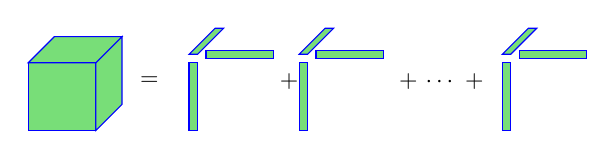
\begin{tikzpicture}[scale=0.215, every node/.style={transform shape}]
		\pgfmathsetmacro{\cubex}{4}
		\pgfmathsetmacro{\cubey}{4}
		\pgfmathsetmacro{\cubez}{4}
		\draw[blue,fill=pastelgreen] (0,0,0) -- ++(-\cubex,0,0) -- ++(0,-\cubey,0) -- ++(\cubex,0,0) -- cycle;
		\draw[blue,fill=pastelgreen] (0,0,0) -- ++(0,0,-\cubez) -- ++(0,-\cubey,0) -- ++(0,0,\cubez) -- cycle;
		\draw[blue,fill=pastelgreen] (0,0,0) -- ++(-\cubex,0,0) -- ++(0,0,-\cubez) -- ++(\cubex,0,0) -- cycle;
		
		\node[draw=none, text=black, scale=4] at (2,-2.25,-3) {$=$};
		\pgfmathsetmacro{\smallwidth}{0.5}
		\draw[blue,fill=pastelgreen] (\cubex+2,0,0) -- ++(-\smallwidth,0,0) -- ++(0,-\cubey,0) -- ++(\smallwidth,0,0) -- cycle;
		\draw[blue,fill=pastelgreen] (\cubex+2 +\cubex + 0.5,0.75,0) -- ++(-\cubex,0,0) -- ++(0,-\smallwidth,0) -- ++(\cubex,0,0) -- cycle;
		\draw[blue,fill=pastelgreen] (\cubex+2,0.5,0) -- ++(-\smallwidth,0,0) -- ++(0,0,-\cubez) -- ++(\smallwidth,0,0) -- cycle;
		
		\node[draw=none, text=black, scale=4] at (2+\cubex+4.25,-2.25,-3) {$+$};
		
		\draw[blue,fill=pastelgreen] (\cubex+2.5 + \cubex+2,0,0) -- ++(-\smallwidth,0,0) -- ++(0,-\cubey,0) -- ++(\smallwidth,0,0) -- cycle;
		\draw[blue,fill=pastelgreen] (\cubex+2.5+\cubex+2 +\cubex + 0.5,0.75,0) -- ++(-\cubex,0,0) -- ++(0,-\smallwidth,0) -- ++(\cubex,0,0) -- cycle;
		\draw[blue,fill=pastelgreen] (\cubex+2.5+\cubex+2,0.5,0) -- ++(-\smallwidth,0,0) -- ++(0,0,-\cubez) -- ++(\smallwidth,0,0) -- cycle;
		
		\node[draw=none, text=black, scale=4] at (2+\cubex+5 + \cubex+ 4.25, -2.25,-3) {$+$ $\cdots$ $+$};
		
		\draw[blue,fill=pastelgreen] (12 + \cubex+2.5 + \cubex+2,0,0) -- ++(-\smallwidth,0,0) -- ++(0,-\cubey,0) -- ++(\smallwidth,0,0) -- cycle;
		\draw[blue,fill=pastelgreen] (12+\cubex+2.5+\cubex+2 +\cubex + 0.5,0.75,0) -- ++(-\cubex,0,0) -- ++(0,-\smallwidth,0) -- ++(\cubex,0,0) -- cycle;
		\draw[blue,fill=pastelgreen] (12 + \cubex+2.5+\cubex+2,0.5,0) -- ++(-\smallwidth,0,0) -- ++(0,0,-\cubez) -- ++(\smallwidth,0,0) -- cycle;
		\end{tikzpicture}
	\end{center}
	\vspace*{-0.15cm}\centering{\footnotesize CP decomposition of a $3$-dimensional tensor.}
	\vfill
	{\footnotesize\vspace*{-0.1cm}$$\T{A}=\sum_{\alpha=1}^{r} U_1 (:,\alpha) \circ U_2(:,\alpha)\circ\cdots \circ U_d(:,\alpha)$$}
%		$$\T{A}(i_1,\cdots,i_d) = \sum_{\alpha=1}^{r} U_1(i_1,\alpha) U_2(i_2,\alpha)\cdots U_d(i_d,\alpha)$$}
	\vfill
	\justifying
	It can be concisely expressed as $\T{A} = \llbracket U_1, U_2, \cdots, U_d \rrbracket$. CP decomposition for a $3$-dimensional tensor in matricized form can be written as:
	$$A_{(1)}=U_1(U_3\odot U_2)^T,\ A_{(2)}=U_2(U_3\odot U_1)^T\ A_{(3)}=U_3(U_2\odot U_1)^T\text.$$
	
	\vfill
	It is useful to assume that $U_1, U_2 \cdots U_d$ are normalized to length one with the weights given in a vector $\lambda \in \mathbb{R}^r$.
	
	$$\T{A} = \llbracket \lambda; U_1, U_2, \cdots, U_d \rrbracket = \sum_{\alpha=1}^{r} \lambda_\alpha U_1 (:,\alpha) \circ U_2(:,\alpha)\circ\cdots \circ U_d(:,\alpha) $$
%	\begin{itemize}
%		\item 
%	\end{itemize}
%	The minimum $r$ required to express $\T{A}$ is called the rank of $\T{A}$. The matrices $U_j \in \mathbb{R}^{n_j\times r}$ for $1\le j \le d$ are called factor matrices.$\qquad\qquad\qquad\qquad\qquad$
%	\vfill
%	\begin{itemize}
%		\item ({\color{green}+}) The number of entries in a CP decomposition of {\footnotesize $\T{A} = \mathcal{O}((n_1+\cdots + n_d)r)$}
%		%		\item ({\color{green}+}) For $n_1=n_2=\cdots n_d=n$, the number of entries = $\mathcal{O}(nrd)$
%		\item ({\color{red}-}) Determining the minimum value of $r$ is an NP-complete problem
%		\item ({\color{red}-}) No robust algorithms to compute this representation
%	\end{itemize}
\end{frame}


\begin{frame}{Tensor rank}
	\small
	$$\T{A} = \sum_{\alpha=1}^{r} \lambda_\alpha U_1 (:,\alpha) \circ U_2(:,\alpha)\circ\cdots \circ U_d(:,\alpha) $$
	
	\begin{itemize}
		\item The minimum $r$ required to express $\T{A}$ is called the rank of $\T{A}$
%		\vfill
%		\item The definition of tensor rank is analogous to the definition of matrix rank
%%		\vfill
	\end{itemize}
The rank of a real-valued tensor may be different over $\mathbb{R}$ and $\mathbb{C}$. For example, consider the frontal slices of $\T{A}\in \mathbb{R}^{2\times 2\times 2}$

$$\T{A}(:,:,1)= \begin{pmatrix}
1 & 0\\
0 & 1
\end{pmatrix} \textnormal{ and } \T{A}(:,:,2) = \begin{pmatrix}
0 & 1\\
-1 & 0
\end{pmatrix}\text .$$
This has rank three over $\mathbb{R}$ and two over $\mathbb{C}$. The CP decomposition over $\mathbb{R}$ has the following factor matrices:
$$U_1=\begin{pmatrix}
1 & 0 & 1\\
0 & 1 & -1
\end{pmatrix}, U_2=\begin{pmatrix}
1 & 0 & 1\\
0 & 1 & 1
\end{pmatrix}, \textnormal{ and } U_3=\begin{pmatrix}
1 & 1 & 0\\
-1 & 1 & 1
\end{pmatrix}\text.$$
The CP decomposition over $\mathbb{C}$ has the following factor matrices:
$$U_1=\frac{1}{\sqrt{2}}\begin{pmatrix}
1 & 1\\
-i & i
\end{pmatrix}, U_2=\frac{1}{\sqrt{2}}\begin{pmatrix}
1 & 1\\
i & -i
\end{pmatrix}, \textnormal{ and } U_3=\begin{pmatrix}
1 & 1\\
i & -i
\end{pmatrix}\text.$$
\end{frame}

\begin{frame}{Rank and low-rank approximations}
\begin{itemize}
	\item Determining the rank of a tensor is an NP-complete problem
	\vfill
	\item If $\T{A} = \sum_{\alpha=1}^{r} \lambda_\alpha U_1 (:,\alpha) \circ U_2(:,\alpha)\circ\cdots \circ U_d(:,\alpha)$, summing $k<r$ terms may not yield a best rank-$k$ approximation
	\vfill
	\item Possible that the best rank-$k$ approximation of a tensor may not exist
\end{itemize}
\end{frame}

\begin{frame}{CP decomposition: example}
	\small
	Let $\T{A} \in \mathbb{R}^{2\times 4\times 3}$ and $A= \llbracket U_1, U_2, U_3\rrbracket$. The rank of $\T{A}$ is $2$.
	$$U_1=\begin{pmatrix} 1& 3\\
	2 & 4
	\end{pmatrix}\text, \quad U_2=\begin{pmatrix}
	1 & 4\\
	2 & 5\\
	4 & 6\\
	3 & 7\\
	\end{pmatrix}\text, \quad U_3=\begin{pmatrix}
	1 & 4\\
	2 & 5\\
	3 & 6
	\end{pmatrix}$$
	\vfill
	Computation of $\T{A}(2,3,1)$,
	\begin{align*}
	\T{A}(2,3,1) =& \sum_{\alpha=1}^{2}U_1(2,\alpha) U_2(3,\alpha)U_3(1,\alpha)\\
	=& 2\cdot 4\cdot 1+4\cdot 6\cdot 4=104 
	\end{align*}
	\vfill
	$\T{A}$ has total 24 elements, while the CP representation has 18 elements.
\end{frame}

\subsection{Computing CP with Alternating Least Squares}
	\begin{frame}{Table of Contents}		
	\tableofcontents[currentsection] % Output the table of contents (all sections on one slide)		
	\end{frame}
\begin{frame}{CP optimization problem for a $3$-dimensional tensor}
	\begin{center}
	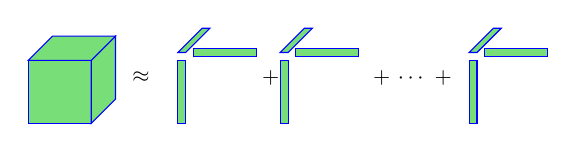
\begin{tikzpicture}[scale=0.2, every node/.style={transform shape}]
	\pgfmathsetmacro{\cubex}{4}
	\pgfmathsetmacro{\cubey}{4}
	\pgfmathsetmacro{\cubez}{4}
	\draw[blue,fill=pastelgreen] (0,0,0) -- ++(-\cubex,0,0) -- ++(0,-\cubey,0) -- ++(\cubex,0,0) -- cycle;
	\draw[blue,fill=pastelgreen] (0,0,0) -- ++(0,0,-\cubez) -- ++(0,-\cubey,0) -- ++(0,0,\cubez) -- cycle;
	\draw[blue,fill=pastelgreen] (0,0,0) -- ++(-\cubex,0,0) -- ++(0,0,-\cubez) -- ++(\cubex,0,0) -- cycle;
	
	\node[draw=none, text=black, scale=4] at (2,-2.25,-3) {$\approx$};
	\pgfmathsetmacro{\smallwidth}{0.5}
	\draw[blue,fill=pastelgreen] (\cubex+2,0,0) -- ++(-\smallwidth,0,0) -- ++(0,-\cubey,0) -- ++(\smallwidth,0,0) -- cycle;
	\draw[blue,fill=pastelgreen] (\cubex+2 +\cubex + 0.5,0.75,0) -- ++(-\cubex,0,0) -- ++(0,-\smallwidth,0) -- ++(\cubex,0,0) -- cycle;
	\draw[blue,fill=pastelgreen] (\cubex+2,0.5,0) -- ++(-\smallwidth,0,0) -- ++(0,0,-\cubez) -- ++(\smallwidth,0,0) -- cycle;
	
	\node[draw=none, text=black, scale=4] at (2+\cubex+4.25,-2.25,-3) {$+$};
	
	\draw[blue,fill=pastelgreen] (\cubex+2.5 + \cubex+2,0,0) -- ++(-\smallwidth,0,0) -- ++(0,-\cubey,0) -- ++(\smallwidth,0,0) -- cycle;
	\draw[blue,fill=pastelgreen] (\cubex+2.5+\cubex+2 +\cubex + 0.5,0.75,0) -- ++(-\cubex,0,0) -- ++(0,-\smallwidth,0) -- ++(\cubex,0,0) -- cycle;
	\draw[blue,fill=pastelgreen] (\cubex+2.5+\cubex+2,0.5,0) -- ++(-\smallwidth,0,0) -- ++(0,0,-\cubez) -- ++(\smallwidth,0,0) -- cycle;
	
	\node[draw=none, text=black, scale=4] at (2+\cubex+5 + \cubex+ 4.25, -2.25,-3) {$+$ $\cdots$ $+$};
	
	\draw[blue,fill=pastelgreen] (12 + \cubex+2.5 + \cubex+2,0,0) -- ++(-\smallwidth,0,0) -- ++(0,-\cubey,0) -- ++(\smallwidth,0,0) -- cycle;
	\draw[blue,fill=pastelgreen] (12+\cubex+2.5+\cubex+2 +\cubex + 0.5,0.75,0) -- ++(-\cubex,0,0) -- ++(0,-\smallwidth,0) -- ++(\cubex,0,0) -- cycle;
	\draw[blue,fill=pastelgreen] (12 + \cubex+2.5+\cubex+2,0.5,0) -- ++(-\smallwidth,0,0) -- ++(0,0,-\cubez) -- ++(\smallwidth,0,0) -- cycle;
	\end{tikzpicture}
\end{center}
For fixed rank $k$, we want to solve
$$\min_{U_1,U_2U_3} ||\T{A} - \sum_{\alpha=1}^{k} \lambda_\alpha U_1(:,\alpha) \circ U_2(:,\alpha)\circ U_3(:,\alpha) ||.$$

\vfill
\begin{itemize}
	\item It is a nonlinear, nonconvex optimization problem
	\vfill
	\item In the matrix case, the SVD provides us the optimal solution
	\vfill
	\item In the tensor case, convergence to optimum not guaranteed
\end{itemize}
\end{frame}

\begin{frame}{Alternating Least Squares (ALS) method}
Fixing all but one factor matrix, we have a linear least squares problem:
$$\min_{\hat{U_1}}||\T{A} - \sum_{\alpha=1}^{k} \hat{U_1}(:,\alpha) \circ U_2(:,\alpha)\circ U_3(:,\alpha)||$$
or equivalently
$$\min_{\hat{U_1}}||A_{(1)} - \hat{U_1}(U_3\odot U_2)^T||$$

\vfill
ALS works by alternating over factor matrices, updating one at a time.
\end{frame}

\begin{frame}{CP-ALS algorithm}
	\small
\textbf{Repeat} until maximum iterations reached or no further improvement obtained
\begin{enumerate}
	\item Solve $U_1(U_3\odot U_2)^T = A_{(1)}$ for $U_1$ $\Rightarrow U_1 = A_{(1)} (U_3\odot U_2) (U_3^TU_3 * U_2^TU_2)^\dagger$
	\item Normalize columns of $U_1$
	\item Solve $U_2(U_3\odot U_1)^T = A_{(2)}$ for $U_2$ $\Rightarrow U_2 = A_{(2)} (U_3\odot U_1) (U_3^TU_3 * U_1^TU_1)^\dagger$
	\item Normalize columns of $U_2$
	\item Solve $U_3(U_2\odot U_1)^T = A_{(3)}$ for $U_3$ $\Rightarrow U_3 = A_{(3)} (U_2\odot U_1) (U_2^TU_2 * U_1^TU_1)^\dagger$
	\item Normalize columns of $U_3$
\end{enumerate}

\bigskip
Here $A^\dagger$ denotes the Moore--Penrose pseudoinverse of $A$. We use the following identity to get expressions for $U_1, U_2$ and $U_3$:
$$(A\odot B)^T(A\odot B) = A^TA * B^TB$$
\end{frame}
\begin{frame}{ALS for computing a CP decomposition}
	\begin{algorithm}[H]{
		\caption{CP-ALS method to compute CP decomposition\label{alg:canonicalals}}
		%%				\caption{HOSVD Algorithm($\X$, $R_1$, $R_2$, $R_3$)}
		\begin{algorithmic}
			\Require input tensor $\T{A}\in \mathbb{R}^{n_1\times \cdots \times n_d}$, desired rank $k$, initial factor matrices $U_j\in \mathbb{R}^{n_j\times k} \textnormal{ for } 1\le j \le d$
			\Ensure $\llbracket \lambda; U_1, \cdots, U_d\rrbracket $ : a rank-$k$ CP decomposition of $\T{A}$
			\Repeat
			\For{$i=1 \text{ to } d$}
			\State $V\gets U_1^\Tra U_1*\cdots*U_{i-1}^\Tra U_{i-1} U_{i+1}^\Tra U_{i+1} *\cdots*U_d^\Tra U_d$
			\State $U_i \gets A_{(i)} (U_d\odot\cdots\odot U_{i+1}\odot U_{i-1}\odot U_1)$\label{alg:canonicalals:mttkrp}
			\State $U_i\gets U_iV^\dagger$ 
			\State $\lambda\gets \text{normalize colums of } U_i$ 
			\EndFor
			\Until converge or the maximum number of iterations
		\end{algorithmic}
}\end{algorithm}

\begin{itemize}
	\item $U_j$ can be chosen randomly or by setting $k$ left singular vectors of $A_{(j)}$ for $1\le j \le d$
\end{itemize}

\end{frame}

\section{Tucker decomposition}
\begin{frame}{Table of Contents}		
	\tableofcontents[currentsection,hideallsubsections] % Output the table of contents (all sections on one slide)		
\end{frame}

\begin{frame}{Tucker decomposition of $\T{A} \in \mathbb{R}^{n_1\times n_2\times\cdots\times n_d}$}
	
	\small
	It represents a tensor with $d$ matrices (usually orthonormal) and a small core tensor.
	\vspace*{-0.25cm}\begin{center}
		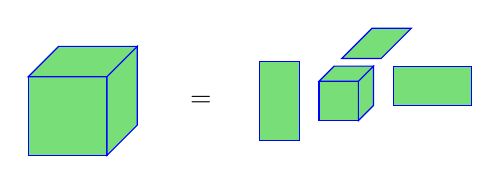
\begin{tikzpicture}[scale=0.25, every node/.style={transform shape}]
		\pgfmathsetmacro{\cubex}{4}
		\pgfmathsetmacro{\cubey}{4}
		\pgfmathsetmacro{\cubez}{4}
		\draw[blue,fill=pastelgreen] (-12,1,\cubez-2) -- ++(-\cubex,0,0) -- ++(0,-\cubey,0) -- ++(\cubex,0,0) -- cycle;
		\draw[blue,fill=pastelgreen] (-12,1,\cubez-2) -- ++(0,0,-\cubez) -- ++(0,-\cubey,0) -- ++(0,0,\cubez) -- cycle;
		\draw[blue,fill=pastelgreen] (-12,1,\cubez-2) -- ++(-\cubex,0,0) -- ++(0,0,-\cubez) -- ++(\cubex,0,0) -- cycle;
		\node[draw=none, text=black, scale=4] at (-8,-1,0) {$=$};
		
		\pgfmathsetmacro{\cubex}{2}
		\pgfmathsetmacro{\cubey}{2}
		\pgfmathsetmacro{\cubez}{2}
		\draw[blue,fill=pastelgreen] (0,0,0) -- ++(-\cubex,0,0) -- ++(0,-\cubey,0) -- ++(\cubex,0,0) -- cycle;
		\draw[blue,fill=pastelgreen] (0,0,0) -- ++(0,0,-\cubez) -- ++(0,-\cubey,0) -- ++(0,0,\cubez) -- cycle;
		\draw[blue,fill=pastelgreen] (0,0,0) -- ++(-\cubex,0,0) -- ++(0,0,-\cubez) -- ++(\cubex,0,0) -- cycle;
		
		\draw[blue,fill=pastelgreen] (-\cubex-1,1,0) -- ++(-\cubex,0,0) -- ++(0,-\cubey-2,0) -- ++(\cubex,0,0) -- cycle;
		\draw[blue,fill=pastelgreen] (\cubex+2+1,0,-\cubey) -- ++(-\cubex-2,0,0) -- ++(0,-\cubey,0) -- ++(\cubex+2,0,0) -- cycle;
		
		\draw[blue,fill=pastelgreen] (0,0,-\cubez-1) -- ++(-\cubex,0,0) -- ++(0,0,-\cubez-2) -- ++(\cubex,0,0) -- cycle;
		\end{tikzpicture}
	\end{center}
			\vspace*{-0.15cm}\centering{\footnotesize Tucker decomposition of a $3$-dimensional tensor.}
			\vfill
			{\footnotesize\vspace*{-0.1cm}$$\T{A} = \T{G} \times_1 U_1 \cdots \times_d U_d$$
			$$\T{A}(i_1,\cdots,i_d) = \sum_{\alpha_1=1}^{r_1}\cdots\sum_{\alpha_d=1}^{r_d} \T{G}(\alpha_1,\cdots,\alpha_d)U_1(i_1,\alpha_1)\cdots U_d(i_d, \alpha_d)$$}
			\vfill
			\justifying
			It can be concisely expressed as $\T{A} = \llbracket \T{G}; U_1, \cdots, U_d\rrbracket $.
			\vfill
			Here $r_j$ for $1\le j\le d$ denote a set of ranks. Matrices $U_j \in \mathbb{R}^{n_j\times r_j}$ for $1\le j \le d$ are usually orthonormal and known as factor matrices. The tensor $\T{G}\in \mathbb{R}^{r_1\times r_2\times\cdots\times r_d}$ is called the core tensor. 
%			\vfill 
%	\begin{itemize}
%		\item ({\color{green}+}) SVD based stable algorithms to compute this decomposition
%		\item ({\color{red}-}) The number of entries = $\mathcal{O}(n_1r_1 + \cdots + n_dr_d+ \prod_{j=1}^{d}r_j)$
%%		\item ({\color{red}-}) For $n_1=n_2=\cdots n_d=n$ and $r_1=r_2=\cdots =r_d=r$, the number of entries = $\mathcal{O}(ndr+r^d)$
%	\end{itemize}	
\end{frame}

\begin{frame}{Tucker decomposition: an example}
\small
Let $\T{A} \in \mathbb{R}^{3\times 3\times 3}$, $\T{G} \in \mathbb{R}^{2\times 2\times 2}$ and $\T{A}=\llbracket\T{G}; U_1, U_2, U_3 \rrbracket$.\footnotesize
\vspace*{-0.1cm}$$U_1 = \frac{1}{3}\begin{pmatrix}
2 & -2\\
1 & 2\\
2 & 1
\end{pmatrix}\text, \quad
U_2=\begin{pmatrix}
1 & 0\\
0 & 1\\
0 & 0
\end{pmatrix}\text, \quad
U_3 = \frac{1}{5}\begin{pmatrix}
0 & 4\\
3 & 3\\
4 & 0
\end{pmatrix}$$
\vspace*{-0.1cm}$$\T{G}(:,:,1)=\begin{pmatrix}
1 & 4\\
2 & 5\\
3 & 6
\end{pmatrix}\text, \qquad\qquad\T{G}(:,:,2)=\begin{pmatrix}
7 & 10\\
8 & 11\\
9 & 12
\end{pmatrix} $$

\vfill
%Computation of $\T{A}(3,2,1)$,
\vspace*{-0.15cm}\begin{align*}
\T{A}(3,2,1) =& \sum_{\alpha_1=1}^{2} \sum_{\alpha_2=1}^{2}\sum_{\alpha_3=1}^{2} \T{G}(\alpha_1, \alpha_2, \alpha_3) U_1(3,\alpha_1)U_2(2,\alpha_2)U_3(1,\alpha_3)\\
=& \T{G}(1,1,1)U_1(3,1)U_2(2,1)U_3(1,1) + \T{G}(1,1,2)U_1(3,1)U_2(2,1)U_3(1,2)\\
 &+ \T{G}(1,2,1)U_1(3,1)U_2(2,2)U_3(1,1)+ \T{G}(1,2,2)U_1(3,1)U_2(2,2)U_3(1,2)\\
 & + \T{G}(2,1,1)U_1(3,2)U_2(2,1)U_3(1,1) + \T{G}(2,1,2)U_1(3,2)U_2(2,1)U_3(1,2)\\
& + \T{G}(2,2,1)U_1(3,2)U_2(2,2)U_3(1,1) + \T{G}(2,2,2)U_1(3,2)U_2(2,2)U_3(1,2)\\
=&1\cdot \frac23 \cdot 0 \cdot 0 + 7\cdot \frac23 \cdot 0 \cdot\frac45+ 4\cdot \frac23 \cdot 1\cdot 0 + 10\cdot \frac23 \cdot 1 \cdot \frac 45 \\
& + 2\cdot \frac13 \cdot 0 \cdot 0 + 8\cdot \frac13 \cdot 0 \cdot\frac 45 + 5\cdot \frac13 \cdot 1 \cdot 0 + 11\cdot \frac 13 \cdot 1 \cdot \frac 45 = \frac{124}{15}\text.
\end{align*}
\end{frame}
\subsection{Computing Tucker decomposition}
\begin{frame}{Table of Contents}		
	\tableofcontents[currentsection] % Output the table of contents (all sections on one slide)		
\end{frame}

\begin{frame}{\large High Order SVD (HOSVD) for computing a Tucker decomposition}
	\small
		\begin{algorithm}[H]{
			\caption{HOSVD method to compute a Tucker decomposition}
			\begin{algorithmic}
				\Require input tensor $\T{A}\in \mathbb{R}^{n_1\times \cdots \times n_d}$, desired rank $(r_1,\cdots, r_d)$
				\Ensure  $\T{A} = \T{G} \times_1 U_1 \times_2 U_2  \cdots \times_d U_d$
				\For{$k=1 \text{ to } d$}
				\State $U_k \gets r_k$ leading left singular vectors of $A_{(k)}$
				\EndFor
				\State $\T{G} = \T{A} \times_1 U_1^\Tra \times_2 U_2^\Tra  \cdots \times_d U_d^\Tra$
			\end{algorithmic}
	}\end{algorithm}


\vfill
\begin{itemize}
	\item When $r_i < rank(A_{(i)})$ for one or more $i$, the decomposition is called the truncated-HOSVD (T-HOSVD)
	\vfill
	\item Output of T-HOSVD can be used as a starting point for an ALS algorithm
\end{itemize}
\end{frame}


\begin{frame}{Quasi-optimality of T-HOSVD}
\small
Let $\tilde{\T{A}} = \T{G} \times_1 U_1 \times_2 U_2  \cdots \times_d U_d$ be the tensor obtained from T-HOSVD.
{\footnotesize
\begin{align*}
||\T{A} - \tilde{\T{A}}||_F^2 =& ||\T{A} -\T{G} \times_1 U_1 \times_2 U_2  \cdots \times_d U_d||_F^2
= ||\T{A} -\T{A} \times_1 U_1U_1^\Tra   \cdots \times_d U_dU_d^\Tra||_F^2\\
=& ||\T{A} -\T{A} \times_1 U_1U_1^\Tra  +\T{A} \times_1 U_1U_1^\Tra  -\T{A} \times_1 U_1U_1^\Tra   \cdots \times_d U_dU_d^\Tra||_F^2\\
=& ||\T{A} -\T{A} \times_1 U_1U_1^\Tra||_F^2 + ||\T{A} \times_1 U_1U_1^\Tra  -\T{A} \times_1 U_1U_1^\Tra   \cdots \times_d U_dU_d^\Tra||_F^2\\
=& ||\T{A} -\T{A} \times_1 U_1U_1^\Tra||_F^2 + ||\T{A} \times_1 U_1U_1^\Tra  - \T{A} \times_1 U_1U_1^\Tra \times_2 U_2U_2^\Tra||_F^2 + \cdots \\
& \cdots + ||\T{A} \times_1 U_1U_1^\Tra   \cdots \times_{d-1} U_{d-1}U_{d-1}^\Tra - \T{A} \times_1 U_1U_1^\Tra \cdots \times_d U_dU_d^\Tra||_F^2\\
\le& ||\T{A} -\T{A} \times_1 U_1U_1^\Tra||_F^2 + ||\T{A} -\T{A} \times_2 U_2U_2^\Tra||_F^2 + \cdots + ||\T{A} -\T{A} \times_d U_dU_d^\Tra||_F^2
\end{align*}\vspace*{-0.65cm}
}
\begin{theorem}
	Tensor $\tilde{\T{A}}$ obtained from T-HOSVD satisfies quasi-optimality condition
	\vspace*{-0.15cm}$$||A-\tilde{\T{A}}||_F \le \sqrt{d} ||\T{A}-\T{A}_{best}||_F\text,$$\vspace*{-0.1cm}
where $\T{A}_{best}$ is the best approximation of $\T{A}$ with ranks $(r_1, \cdots, r_d)$.
\end{theorem}
Proof: $||\T{A} -\T{A} \times_i U_iU_i^\Tra||_F \le ||\T{A}-\T{A}_{best}||_F $ for $1\le i \le d$.  Substituting these in the previous result yields the specified inequality.
\vfill
\end{frame}
\begin{frame}{\large Sequentially T-HOSVD (ST-HOSVD) for Tucker decomposition}
	\small
	\begin{itemize}
		\item This method is more work efficient than T-HOSVD
		\vfill
		\item In each step, it reduces the size of one dimension of the tensor
	\end{itemize}
	
	%	\small
	\begin{algorithm}[H]{
			\caption{ST-HOSVD method to compute a Tucker decomposition}
			\begin{algorithmic}
				\Require input tensor $\T{A}\in \mathbb{R}^{n_1\times \cdots \times n_d}$, desired rank $(r_1,\cdots, r_d)$
				\Ensure  $\llbracket \T{G}; U_1, \cdots, U_d\rrbracket $ : a $(r_1, \cdots, r_d)$-rank Tucker decomposition of $\T{A}$
				\State $\T{B} \gets \T{A}$
				\For{$k=1 \text{ to } d$}
				\State $S\gets B_{(k)}B_{(k)}^T$
				\State $U_k \gets r_k$ leading eigen vectors of $S$
				\State $\T{B} \gets \T{B} \times_i U_i$
				\EndFor
				\State $\T{G} = \T{A} \times_1 U_1^\Tra \times_2 U_2^\Tra \cdots \times_d U_d^\Tra$
			\end{algorithmic}
	}\end{algorithm}
	
	
%	\vfill
%	\begin{itemize}
%		\item When $r_i < rank(A_{(i)})$ for one or more $i$, the decomposition is called the truncated-HOSVD (T-HOSVD)
%		\vfill
%		\item Output of T-HOSVD can be used as a starting point for an ALS algorithm
%	\end{itemize}
\end{frame}

\begin{frame}{Quasi-optimality of ST-HOSVD}
	\small
	Let $\tilde{\T{A}} = \T{G} \times_1 U_1 \times_2 U_2  \cdots \times_d U_d$ be the tensor obtained from ST-HOSVD.
	{\footnotesize
		\begin{align*}
		||\T{A} - \tilde{\T{A}}||_F^2 =& ||\T{A} -\T{G} \times_1 U_1 \times_2 U_2  \cdots \times_d U_d||_F^2
		= ||\T{A} -\T{A} \times_1 U_1U_1^\Tra   \cdots \times_d U_dU_d^\Tra||_F^2\\
		=& ||\T{A} -\T{A} \times_1 U_1U_1^\Tra||_F^2 + ||\T{A} \times_1 U_1U_1^\Tra  - \T{A} \times_1 U_1U_1^\Tra \times_2 U_2U_2^\Tra||_F^2 + \cdots \\
		& \cdots + ||\T{A} \times_1 U_1U_1^\Tra   \cdots \times_{d-1} U_{d-1}U_{d-1}^\Tra - \T{A} \times_1 U_1U_1^\Tra \cdots \times_d U_dU_d^\Tra||_F^2
		\end{align*}\vspace*{-0.65cm}
	}
	\begin{theorem}
		\vspace*{-0.1cm}Tensor $\tilde{\T{A}}$ obtained from ST-HOSVD satisfies quasi-optimality condition
		\vspace*{-0.15cm}$$||A-\tilde{\T{A}}||_F \le \sqrt{d} ||\T{A}-\T{A}_{best}||_F\text,$$\vspace*{-0.1cm}
		where $\T{A}_{best}$ is the best approximation of $\T{A}$ with ranks $(r_1, \cdots, r_d)$.
	\end{theorem}
	Proof: We know that $||\T{A} -\T{A} \times_i U_iU_i^\Tra||_F \le ||\T{A}-\T{A}_{best}||_F $ for $1\le i \le d$.
	{\footnotesize
		$$||\T{A} -\T{A} \times_1 U_1U_1^\Tra||_F   \le ||\T{A}-\T{A}_{best}||_F$$
		$$||\T{A} \times_1 U_1U_1^\Tra  - \T{A} \times_1 U_1U_1^\Tra \times_2 U_2U_2^\Tra||_F  \le ||\T{A} -\T{A} \times_2 U_2U_2^\Tra||_F  \le ||\T{A}-\T{A}_{best}||_F$$
		{\tiny $$\vdots$$}
		{\scriptsize \vspace*{-0.5cm}$$||\T{A} \times_1 U_1U_1^\Tra   \cdots \times_{d-1} U_{d-1}U_{d-1}^\Tra - \T{A} \times_1 U_1U_1^\Tra \cdots \times_d U_dU_d^\Tra||_F  \le ||\T{A} -\T{A} \times_d U_dU_d^\Tra||_F  \le ||\T{A}-\T{A}_{best}||_F$$}
}
Summing the above terms yields the specified inequality.
\vfill
\end{frame}

\begin{frame}{\large Tucker decomposition optimization problem for a $3$-dimensional tensor}
	\begin{center}
	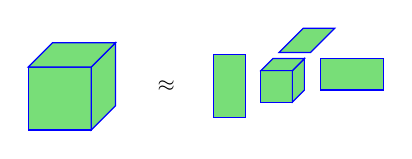
\begin{tikzpicture}[scale=0.2, every node/.style={transform shape}]
	\pgfmathsetmacro{\cubex}{4}
	\pgfmathsetmacro{\cubey}{4}
	\pgfmathsetmacro{\cubez}{4}
	\draw[blue,fill=pastelgreen] (-12,1,\cubez-2) -- ++(-\cubex,0,0) -- ++(0,-\cubey,0) -- ++(\cubex,0,0) -- cycle;
	\draw[blue,fill=pastelgreen] (-12,1,\cubez-2) -- ++(0,0,-\cubez) -- ++(0,-\cubey,0) -- ++(0,0,\cubez) -- cycle;
	\draw[blue,fill=pastelgreen] (-12,1,\cubez-2) -- ++(-\cubex,0,0) -- ++(0,0,-\cubez) -- ++(\cubex,0,0) -- cycle;
	\node[draw=none, text=black, scale=4] at (-8,-1,0) {$\approx$};
	
	\pgfmathsetmacro{\cubex}{2}
	\pgfmathsetmacro{\cubey}{2}
	\pgfmathsetmacro{\cubez}{2}
	\draw[blue,fill=pastelgreen] (0,0,0) -- ++(-\cubex,0,0) -- ++(0,-\cubey,0) -- ++(\cubex,0,0) -- cycle;
	\draw[blue,fill=pastelgreen] (0,0,0) -- ++(0,0,-\cubez) -- ++(0,-\cubey,0) -- ++(0,0,\cubez) -- cycle;
	\draw[blue,fill=pastelgreen] (0,0,0) -- ++(-\cubex,0,0) -- ++(0,0,-\cubez) -- ++(\cubex,0,0) -- cycle;
	
	\draw[blue,fill=pastelgreen] (-\cubex-1,1,0) -- ++(-\cubex,0,0) -- ++(0,-\cubey-2,0) -- ++(\cubex,0,0) -- cycle;
	\draw[blue,fill=pastelgreen] (\cubex+2+1,0,-\cubey) -- ++(-\cubex-2,0,0) -- ++(0,-\cubey,0) -- ++(\cubex+2,0,0) -- cycle;
	
	\draw[blue,fill=pastelgreen] (0,0,-\cubez-1) -- ++(-\cubex,0,0) -- ++(0,0,-\cubez-2) -- ++(\cubex,0,0) -- cycle;
	\end{tikzpicture}
\end{center}
\justifying
For fixed ranks orthonormal matrices $U_1, U_2, U_3$, we want to solve
$$\min_{U_1,U_2,U_3} ||\T{A} - \T{G} \times_1 U_1 \times_2 U_2 \times_3 U_3|| \textnormal {, where } \T{G}=\T{A}\times_1 U_1^T \times_2 U_2^T \times_3 U_3^T \text.$$
\vfill
This is equivalent to
$$\max_{U_1,U_2,U_3} ||\T{A}\times_1 U_1^T \times_2 U_2^T \times_3 U_3^T ||\text.$$

It is a nonlinear, nonconvex optimization problem.
\end{frame}
\begin{frame}{Higher-order orthogonal iteration (HOOI) method}
	Fixing all but one factor matrix, we have a matrix problem:
	$$\max_{\hat{U_1}} ||\T{A}\times_1 \hat{U_1}^T \times_2 U_2^T \times_3 U_3^T ||$$
	
	\vfill
	HOOI works by alternating over factor matrices, updating one by computing left singular vectors
\end{frame}


\begin{frame}{HOOI method for computing a Tucker decomposition}
	\small
	\begin{algorithm}[H]{
			\caption{HOOI method to compute Tucker decomposition}
			\begin{algorithmic}
				\Require input tensor $\T{A}\in \mathbb{R}^{n_1\times \cdots \times n_d}$, desired ranks $(r_1, \cdots, r_d)$, initial factor matrices $U_j\in \mathbb{R}^{n_j\times r_j} \textnormal{ for } 1\le j \le d$
				\Ensure $\llbracket \T{G}; U_1, \cdots, U_d\rrbracket $ : a $(r_1, \cdots, r_d)$-rank Tucker decomposition of $\T{A}$
				\Repeat
				\For{$i=1 \text{ to } d$}
				\State $\T{B} \gets \T{A}\times_1 U_1^T  \cdots \times_{i-1} U_{i-1}^T \times_{i+1} U_{i+1}^T \cdots \times_d U_d^T$
				\State $U_i\gets$ $r_i$ left singular vectors of $B_{(i)}$
				\EndFor
				\Until converge or the maximum number of iterations
				\State $\T{G} \gets \T{A}\times_1 U_1^T \times_2 U_2^T \cdots  \times_d U_d^T$
			\end{algorithmic}
	}\end{algorithm}
	
	\vfill
	\begin{itemize}
		\item  Outputs of HOSVD ($U_j$ for $1\le j \le d$) can be used as a starting point for this method 
	\end{itemize}
	
\end{frame}


\section{Tensor Train decomposition}
\begin{frame}{Table of Contents}		
	\tableofcontents[currentsection,hideallsubsections] % Output the table of contents (all sections on one slide)		
\end{frame}

%------------------------------------------------
\begin{frame}{\large Tensor Train (TT) decomposition: Product of matrices view}
	
	\small
	\begin{itemize}
		\item A $d$-dimensional tensor is represented with $2$ matrices and $d$-$2$ $3$-dimensional tensors.
	\end{itemize}
	\begin{figure}
		\begin{center}	
			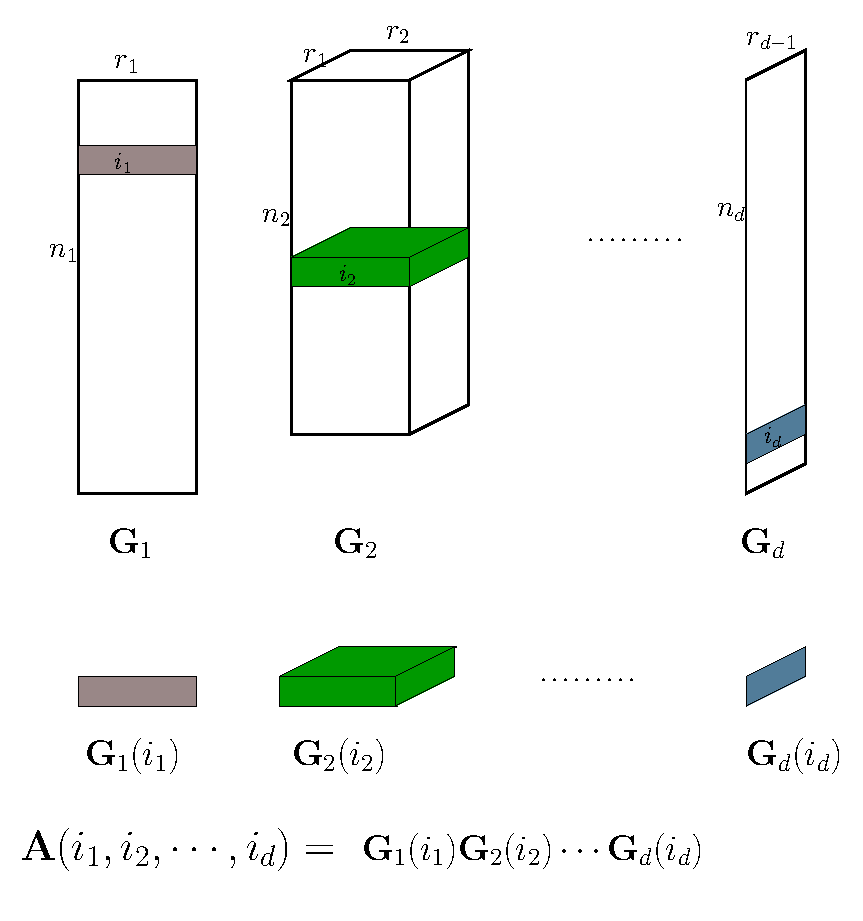
\includegraphics[scale=0.325]{./ttentry.eps}
		\end{center}
	\end{figure}
	\noindent An entry of $\T{A}$ $\in$ $\mathbb{R}^{n_1 \times \cdots \times n_d}$ is computed by multiplying corresponding matrix (or row/column) of each matrix/tensor.
\end{frame}

\begin{frame}{Tensor Train decomposition}
	
	\begin{block}{}
		$\T{A}$ $\in$ $\mathbb{R}^{n_1 \times \cdots \times n_d}$ is represented with cores $\T{G}_k$$\in$ $\mathbb{R}^{r_{k-1}\times n_k\times r_k}$, $k$=$1,2,\cdots d$, $r_0$=$r_d$=$1$ and its elements satisfy the following expression:
		{\small\begin{align*}
			\T{A}(i_1,\cdots ,i_d) 
			&= \sum_{\alpha_0 = 1}^{r_0} \cdots \sum_{\alpha_d = 1}^{r_d} \T{G}_1(\alpha_0, i_1, \alpha_1) \cdots \T{G}_d(\alpha_{d-1}, i_d, \alpha_d)\\
			&= \sum_{\alpha_1 = 1}^{r_1} \cdots \sum_{\alpha_{d-1} = 1}^{r_{d-1}} \T{G}_1(1, i_1, \alpha_1) \cdots \T{G}_d(\alpha_{d-1}, i_d, 1)
			\end{align*}}
		\begin{center}
			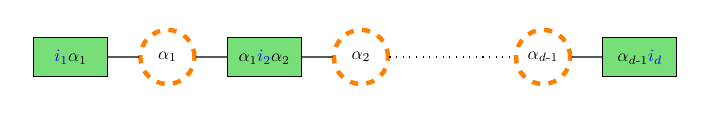
\begin{tikzpicture}[scale=0.625, every node/.style={transform shape}]
			\tikzstyle{taskc}=[circle, draw=orange, minimum size=11mm, fill=none, dashed, ultra thick]
			\tikzstyle{taskr}=[draw=black, minimum height=8mm, minimum width=15mm, anchor=south west, fill=pastelgreen, text=black]
			
			\node(t1) at (0,0) {};
			\node [above right=0cm and 0cm of t1.mid,taskr](T1) {$\textcolor{blue}{i_1}\alpha_1$};
			\node [above right=0cm and 0.8cm of T1.south east, taskc](C1) {$\alpha_1$};
			\node [above right=0cm and 0.8cm of C1.south east, taskr](T2) {$\alpha_1\textcolor{blue}{i_2}\alpha_2$};
			\node [above right=0cm and 0.8cm of T2.south east, taskc](C2) {$\alpha_2$};
			
			\node [above right=0cm and 4.5cm of T2.south east, taskc](Cd) {$\alpha_{d\text{-}1}$};
			\node [above right=0cm and 0.8cm of Cd.south east, taskr](Td) {$\alpha_{d\text{-}1}\textcolor{blue}{i_d}$};
			\draw (T1.east)--(C1.west);
			\draw (C1.east)--(T2.west);
			\draw (T2.east)--(C2.west);
			\draw [dotted] (C2.east)--(Cd.west);
			\draw (Cd.east)--(Td.west);
			\path (-0.1, -0.4) -- (2.5, -0.4); 
			%%\path (-0.1, -0.8) -- (2.5, -0.8); 
			\end{tikzpicture}
		\end{center}
	\end{block}
The ranks $r_k$ are called TT-ranks.
	\begin{itemize}
		\item The number of entries in this decomposition = $\mathcal{O}(n_1r_1 + n_2r_1r_2 + n_3r_2r_3+\cdots + n_{d-1}r_{d-2}r_{d-1} + n_dr_{d-1})$
%		\item For $n_1=n_2=\cdots=n_d=n$ and $r_1=r_2=\cdots=r_{d-1}=r$, the number of entries = $\mathcal{O}(ndr^2)$
	\end{itemize}
\end{frame}
\begin{frame}{TT-decomposition: an example}
	\small
	Let $\T{A} \in \mathbb{R}^{3\times 4\times 5}$, $\T{G} \in \mathbb{R}^{2\times 2\times 2}$. $\T{G}_1 \in\mathbb{R}^{3\times 2}, \T{G}_2 \in\mathbb{R}^{2\times 4\times 2}$, and $\T{G}_3 \in\mathbb{R}^{2\times 5}$ are the cores of a TT-decomposition.
	$$\T{G}_1=\begin{pmatrix}
	1 & 1\\
	2 & 1\\
	3 & 1
	\end{pmatrix}\text, \quad \T{G}_3=\begin{pmatrix}
	1 & 2 & 3 & 4 & 5\\
	1 & 1 & 1 & 1 & 1
	\end{pmatrix}\text,$$
	$$\T{G}_2(:,1,:)=\begin{pmatrix}
	1 & 1\\
	2 & 1
	\end{pmatrix}\text,
	\T{G}_2(:,2,:)=\begin{pmatrix}
	1 & 1\\
	3 & 1
	\end{pmatrix}\text,
	\T{G}_2(:,3,:)=\begin{pmatrix}
	1 & 1\\
	4 & 1
	\end{pmatrix}\text,
	\T{G}_2(:,4,:)=\begin{pmatrix}
	1 & 1\\
	5 & 1
	\end{pmatrix}$$
	\vfill
	Computation of $\T{A}(2,3,4)$,
	\begin{align*}
	\T{A}(2,3,4) = & \T{G}_1(2,:)\T{G}_2(:,3,:)\T{G}_3(,4)\\
	=& \begin{pmatrix} 2 & 1
	\end{pmatrix}\begin{pmatrix} 1 & 1\\ 4 & 1
	\end{pmatrix}\begin{pmatrix} 4\\1
	\end{pmatrix}=27
	\end{align*}
\end{frame}

\begin{frame}{Another representation of unfolding matrices of a tensor}
\small
$A_k$ denotes $k$-th unfolding matrix of tensor $\T{A}$ $\in$ $\mathbb{R}^{n_1 \times \cdots \times n_d}$.

$$ A_k = [A_k(i_1, i_2,\cdots, i_k; i_{k+1},\cdots ,i_d)]$$

\vfill	
	\begin{itemize}
		\item Size of $A_k$ is $(\prod_{\ell=1}^{k}n_\ell)\times(\prod_{\ell = k+1}^{d}n_\ell)$
%		\item $r_k$ denotes the rank of $A_k$
	\end{itemize}

%\begin{itemize}
%	\item ($r_1, r_2,\cdots, r_{d-1}$) denotes the ranks of unfolding matrices of the tensor
%\end{itemize}
\end{frame}

\begin{frame}{TT-SVD algorithm for TT approximation [Oseledets, 2011]}
	\small
	\vspace*{-0.25cm}\begin{algorithm}[H]
		\caption{TT-SVD algorithm}
		\begin{algorithmic}[1]
			\Require $d$-dimensional tensor $\T{A}$ and desired ranks ($r_1, r_2,\cdots r_{d-1}$) 
			\Ensure Cores $\T{G}_k(\alpha_{k-1}, n_k, \alpha_k) _{1\le k\le d}$ of a TT representation with $\alpha_k \le r_k$ and $\alpha_0 = \alpha_d=1$
			\State Temporary tensor: $\T{C} = \T{A}$, $\alpha_0=1$
			\For{$k=1:d-1$}
			\State $A_k$ = $reshape(\T{C}, \alpha_{k-1}n_{k} , \frac{numel(\T{C})}{\alpha_{k-1}n_{k}})$
			\State Compute SVD: $A_k = U \Sigma V^T$
			\State Compute rank of $\Sigma$, $\alpha_k=$ rank($\Sigma$)
			\State New core: $\T{G}_k$ := $reshape(U(;1:\alpha_k), \alpha_{k-1}, n_k, \alpha_k)$
			\State $\T{C}$ = $\Sigma(1:\alpha_k; 1:\alpha_k)V^T(1:\alpha_k;)$
			\EndFor
			\State $\T{G}_d = \T{C}$, $\alpha_{d}=1$
			\State return $\T{G}_1,\cdots,\T{G}_d$
		\end{algorithmic}
	\end{algorithm}
%\vfill
\vspace*{-0.315cm}{\color{blue}$\bullet$} $reshape(A,m_1,\cdots,m_l)$: rearranges array $A$ into a $m_1\times \cdots\times m_d$ array\\ 
{\color{blue}$\bullet$} $numel(A)$: number of elements of array $A$ 
\vfill
\end{frame}
\begin{frame}{Error with TT-SVD approximation}
\small
Suppose the unfolding matrices of $\T{A}$ satisfy the following:
\vspace*{-0.15cm}$$A_k = R_k+E_k \text, \quad R_k \textnormal{ is best $r_k$- rank approximation of }A_k, \quad \textnormal{for } 1\le k \le d-1\text.$$


\vfill
The accuracy analysis of TT-SVD is similar to that of ST-HOSVD method (see [Oseledets, 2011]).

\vfill
Tensor $\T{B}$ obtained from the TT-SVD algorithm satisfies $$||\T{A}-\T{B}||_F^2 = \sum_{k=1}^{d-1}||E_k||_F^2 \text.$$
\vfill
\vspace*{-0.25cm}\begin{theorem}
	\vspace*{-0.1cm}Tensor $\T{B}$ obtained from TT-SVD satisfies quasi-optimality condition
	\vspace*{-0.15cm}$$||A-\T{B}||_F \le \sqrt{d-1} ||\T{A}-\T{A}_{best}||_F\text,$$\vspace*{-0.1cm}
	where $\T{A}_{best}$ is the best $(r_1, \cdots, r_{d-1})$-ranks approximation of $\T{A}$ in TT-format.
\end{theorem}
Proof: As SVD gives the best $r_k$ rank approximation for $A_k$, we have {\footnotesize $$||E_k||_F \le ||\T{A}-\T{A}_{best}||_F \text{ for } 1\le k \le d \text.$$}

\vspace*{-0.45cm}Putting the values of $||E_k||_F$ in the error expression of TT-SVD algorithm completes the proof.
\end{frame}

\begin{frame}{Why TT representation is good for high dimension tensors?}
\small
This representation allows one to perform various basic linear algebra operations in its own structure.
\begin{itemize}
	\item \emph{Addition}: The addition of two tensors in the TT-representation ,
	$$\T{A}=\T{A}_1(i_1)\cdots \T{A}_d(i_d), \quad \T{B}=\T{B}_1(i_1)\cdots \T{B}_d(i_d)\text,$$
	requires to merge core for each mode. Auxiliary dimensions are added. The cores $\T{C}_k(i_k)$ of $\T{C}=\T{A}+\T{B}$ are defined as
	$$\T{C}_k(i_k) = \begin{pmatrix}
	\T{A}_k(i_k) & 0\\
	0 & \T{B}_k(i_k)
	\end{pmatrix}\text, \quad \text{ for } 2\le k\le d-1 \text{, and}$$
	$$\T{C}_1(i_1) = \begin{pmatrix}\T{A}_1(i_1) & \T{B}_1(i_1)\end{pmatrix}\text, \quad  \T{C}_d(i_d) = \begin{pmatrix}\T{A}_d(i_d)\\  \T{B}_d(i_d)\end{pmatrix}\text.$$
	\item \emph{Multiplication by a number}: requires to scale one of the cores
	\item Multidimensional contraction, Hadamard product  and scalar product can also be performed
	\item Further approximation (or compression) can also be obtained
\end{itemize}
\end{frame}
\section{Compact representations of tensor operations}
\begin{frame}{Table of Contents}		
	\tableofcontents[currentsection,hideallsubsections] % Output the table of contents (all sections on one slide)		
\end{frame}
\begin{frame}{Tensor network representations}
\small
Notation: Tensors are denoted by solid shapes and number of lines denote the dimensions of the tensors. Connecting two lines implies summation (or contraction) over the connected dimensions.


\vfill

\begin{tabular}{cc}
	Vector : & 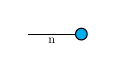
\begin{tikzpicture}[scale=0.45, every node/.style={transform shape}]
	\tikzstyle{taskc}=[circle, draw=black, minimum size=3mm, fill=\tensorcolor]
	\node (t01) at (0,0) [taskc]{};
	\draw (t01) -- node[below] {n} (-1.5,0);
	\end{tikzpicture}\\
	&\\
	Matrix : & 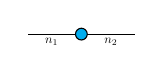
\begin{tikzpicture}[scale=0.45, every node/.style={transform shape}]
	\tikzstyle{taskc}=[circle, draw=black, minimum size=3mm, fill=\tensorcolor]
	\node (t01) at (0,0) [taskc]{};
	\draw (t01) -- node[below] {$n_1$} (-1.5,0);
	\draw (t01) -- node[below] {$n_2$} (1.5,0);
	\end{tikzpicture}\\
	&\\
	3-dimensional tensor : & 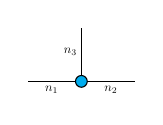
\begin{tikzpicture}[scale=0.45, every node/.style={transform shape}]
	\tikzstyle{taskc}=[circle, draw=black, minimum size=3mm, fill=\tensorcolor]
	\node (t01) at (0,0) [taskc]{};
	\draw (t01) -- node[below] {$n_1$} (-1.5,0);
	\draw (t01) -- node[below] {$n_2$} (1.5,0);
	\draw (t01) -- node[left] {$n_3$} (0,1.5);
	\end{tikzpicture}\\
	Tucker decomposition of a $3$-dimensional tensor : & 
	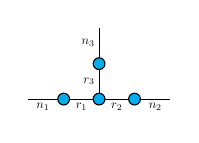
\begin{tikzpicture}[scale=0.45, every node/.style={transform shape}]
	\tikzstyle{taskc}=[circle, draw=black, minimum size=3mm, fill=\tensorcolor]
	\node (t0) at (0,0) [taskc]{};
	\node (t1) at (-1,0) [taskc]{};
	\node (t2) at (1,0) [taskc]{};
	\node (t3) at (0, 1) [taskc]{};
	
	\draw (t1) --node[below] {$r_1$} (t0);
	\draw (-2,0) --node[below] {$n_1$} (t1);
	
	\draw (t0) --node[below] {$r_2$} (t2);
	\draw (t2) --node[below] {$n_2$} (2,0);
	
	\draw (t0) --node[left] {$r_3$} (t3);
	\draw (t3) --node[left] {$n_3$} (0,2);
	\end{tikzpicture}\\
	& \\
	TT decomposition of of a $4$-dimensional tensor &
	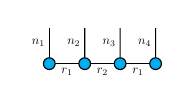
\begin{tikzpicture}[scale=0.45, every node/.style={transform shape}]
	\tikzstyle{taskc}=[circle, draw=black, minimum size=3mm, fill=\tensorcolor]
	\node (t0) at (0,0) [taskc]{};
	\node (t1) at (1,0) [taskc]{};
	\node (t2) at (2,0) [taskc]{};
	\node (t3) at (3,0) [taskc]{};
	
	\draw (t0) --node[left] {$n_1$} (0,1);
	\draw (t1) --node[left] {$n_2$} (1,1);
	\draw (t2) --node[left] {$n_3$} (2,1);
	\draw (t3) --node[left] {$n_4$} (3,1);
	
	
	\draw (t0) --node[below] {$r_1$} (t1);
	\draw (t1) --node[below] {$r_2$} (t2);
	\draw (t2) --node[below] {$r_1$} (t3);
	\end{tikzpicture}
\end{tabular}

\end{frame}



%
%\begin{frame}{Strassen's algorithm for matrix multiplication ($C= AB$)}
%	\begin{itemize}
%		%%	\item $C= AB$, where $A \in\mathbb{R}^{m \times k}$, $B \in\mathbb{R}^{k \times n}$, and  $C$ $\in$ $\mathbb{R}^{m \times n}$
%		\item Matrix is divided into 2$\times$2 blocks
%	\end{itemize}
%	\begin{align*}
%	\begin{pmatrix}
%	C_{11} & C_{12} \\
%	C_{21} & C_{22}
%	\end{pmatrix}
%	&
%	=
%	\begin{pmatrix}
%	A_{11} & A_{12} \\
%	A_{21} & A_{22}
%	\end{pmatrix}
%	\begin{pmatrix}
%	B_{11} & B_{12} \\
%	B_{21} & B_{22}
%	\end{pmatrix}
%	\end{align*}
%	
%	\begin{minipage}{0.45\columnwidth}
%		\begin{align*}\small
%		M_1 &= (A_{11} + A_{22})(B_{11}+B_{22})\\
%		M_2 &= (A_{21} + A_{22})B_{11}\\
%		M_3 &= A_{11} (B_{12}-B_{22})\\
%		M_4 &= A_{22} (B_{21}-B_{11})\\
%		M_5 &= (A_{11} +A_{12})B_{22}\\
%		M_6 &= (A_{21}-A_{11})(B_{11} +B_{12})\\
%		M_7 &= (A_{12}-A_{22})(B_{21} + B_{22}) 
%		\end{align*}
%	\end{minipage}
%	\hfill
%	\begin{minipage}{0.45\columnwidth}
%		\begin{center}
%			\begin{align*}
%			C_{11} &= M_1 + M_4 -M_5 +M_7\\
%			C_{12} &= M_3 + M_5\\
%			C_{21} &= M_2 + M_4\\
%			C_{22} &= M_1 -M_2 + M_3 + M_6
%			\end{align*}
%		\end{center}
%	\end{minipage}
%	
%\end{frame}
%
%
%
%\begin{frame}{$2\times 2$ matrix multiplication as a tensor operation}
%	\begin{align*}
%	\begin{pmatrix}
%	C_{11} & C_{12} \\
%	C_{21} & C_{22}
%	\end{pmatrix}
%	&
%	=
%	\begin{pmatrix}
%	A_{11} & A_{12} \\
%	A_{21} & A_{22}
%	\end{pmatrix}
%	\begin{pmatrix}
%	B_{11} & B_{12} \\
%	B_{21} & B_{22}
%	\end{pmatrix}
%	\end{align*}
%	
%	We can write this multiplication as a tensor operation,
%	\begin{align*}
%	\tensor{T}\times_1 \begin{pmatrix}
%	A_{11}\\
%	A_{12}\\
%	A_{21}\\
%	A_{22}
%	\end{pmatrix}
%	\times_2 \begin{pmatrix}
%	B_{11}\\
%	B_{12}\\
%	B_{21}\\
%	B_{22}
%	\end{pmatrix}
%	&=\begin{pmatrix}
%	C_{11}\\
%	C_{12}\\
%	C_{21}\\
%	C_{22}
%	\end{pmatrix}
%	\end{align*}
%	Where \tensor{T} is a $4\times4\times4$ tensor with the following slices:
%	\begin{align*}\tiny
%	T_1= \begin{pmatrix}
%	1&0&0&0\\
%	0&0&1&0\\
%	0&0&0&0\\
%	0&0&0&0
%	\end{pmatrix}
%	&\tiny
%	T_2= \begin{pmatrix}
%	0&1&0&0\\
%	0&0&0&1\\
%	0&0&0&0\\
%	0&0&0&0
%	\end{pmatrix}
%	&\tiny
%	T_3= \begin{pmatrix}
%	0&0&0&0\\
%	0&0&0&0\\
%	1&0&0&0\\
%	0&0&1&0
%	\end{pmatrix}
%	&\tiny
%	T_4= \begin{pmatrix}
%	0&0&0&0\\
%	0&0&0&0\\
%	0&1&0&0\\
%	0&0&0&1
%	\end{pmatrix}
%	\end{align*}
%\end{frame}
\end{document} 